% Created 2016-05-04 Wed 17:46
\documentclass[10pt,oneside,x11names]{article}
\usepackage[utf8]{inputenc}
\usepackage[T1]{fontenc}
\usepackage{fixltx2e}
\usepackage{graphicx}
\usepackage{grffile}
\usepackage{longtable}
\usepackage{wrapfig}
\usepackage{rotating}
\usepackage[normalem]{ulem}
\usepackage{amsmath}
\usepackage{textcomp}
\usepackage{amssymb}
\usepackage{capt-of}
\usepackage{hyperref}
\usepackage{geometry}
\usepackage{amsmath}
\usepackage{amssymb}
\usepackage{amsfonts}
\usepackage{palatino}
\usepackage{siunitx}
\usepackage{esdiff}
\usepackage{xfrac}
\usepackage{nicefrac}
\usepackage{faktor}
\usepackage[euler-digits,euler-hat-accent]{eulervm}
\author{Brian Beckman}
\date{\textit{<2016-05-04 Wed>}}
\title{Kalman Folding, Part 1 (REVIEWER'S DRAFT)\\\medskip
\large Extracting Models from Data, One Observation at a Time}
\hypersetup{
 pdfauthor={Brian Beckman},
 pdftitle={Kalman Folding (REVIEWER'S DRAFT)},
 pdfkeywords={},
 pdfsubject={},
 pdfcreator={Emacs 24.5.1 (Org mode 8.3.4)}, 
 pdflang={English}}
\begin{document}

\maketitle
\setcounter{tocdepth}{3}
\tableofcontents


\section{Abstract}
\label{sec:orgheadline1}

Kalman filtering is commonplace in engineering, but less familiar to software
developers. It is the central tool for estimating states of a model, one
observation at a time. It runs fast in constant memory. It is the mainstay of
tracking and navigation, but it is equally applicable to econometrics,
recommendations, control: any application where we update models over time.

By writing a Kalman filter as a functional fold, we can test code in friendly
environments and then deploy identical code with confidence in unfriendly
environments. In friendly environments, data are deterministic, static, and
present in memory. In unfriendly, real-world environments,
data are unpredictable, dynamic, and arrive asynchronously.

The flexibility to deploy exactly the code that was tested is especially
important for numerical code like filters. Detecting, diagnosing and correcting
numerical issues without repeatable data sequences is impractical. Once code is
hardened, it can be critical to deploy exactly the same code, to the binary
level, in production, because of numerical brittleness. Functional form makes it
easy to test and deploy exactly the same code because it minimizes the coupling
between code and environment.

\section{Applications of Kalman Filtering}
\label{sec:orgheadline2}

Kalman filtering estimates states of a linear model from noisy observations. The
most common example is the \emph{tracking problem}. We need to know the position,
attitude, and dynamics of a vehicle so we can predict its trajectory, but we can
only observe radar time-of-flight and angles. We write a model that goes the
other way and predicts radar observations from states, then statistically invert
the model by incrementally accumulating observations. An active variant of
tracking is \emph{navigation}, where we control the vehicle by moving it from its
estimated path to a desired path.

However, Kalman filtering and its many variants are much more broadly
applicable, and this fact is perhaps under-appreciated in the computing
mainstream. We can profitably apply such methods to any problem that fulfills
the following criteria:

\begin{itemize}
\item we have a model that predicts observations from states
\item we accumulate observations and want estimates of the states, that is, we want
to invert the model
\item estimation is continual; observations accumulate over time
\item estimates must include uncertainty information
\item uncertainty of the estimates decreases as observations accumulate
\item the number of observations is unlimited
\item computer memory cannot grow as observations accumulate
\end{itemize}

\noindent Some applications that come to mind include

\begin{description}
\item[{Battery charging}] we have a model that predicts voltage from internal charge
state. We observe voltage and estimate internal charge state to avoid
over-charging and over-discharging the battery.
\item[{Tectonic drift and radio interferometry}] we have a model that predicts
celestial positions of radio sources like quasars and satellites given
geospatial positions of radio telescopes. We observe celestial positions
iterferometrically and solve for geospatial positions and velocities of the
telescopes. Over time, we can see tectonic drift of inter-telescope
baselines.\footnote{JPL Geodynamics Program \url{http://www.jpl.nasa.gov/report/1981.pdf}}
\item[{Recommendations}] we have a model that predicts customer's pages views and
purchases (\emph{conversions}) given the customer's interests. We observe the
customer's page views and conversions and solve for the customer's
interests. As observations accumulate, recommendations based on probability
of future views and purchases improve.
\item[{Capacity planning}] we have models that predict shipping rate, queue depth
and latency, and package-network bandwidths from warehouse and
transportation capacity. We observe shipping rates, queue depth and
latency, and package-network bandwidths and solve for warehouse and
transportation capacities to pinpoint bottlenecks and prioritize
capital improvements.
\item[{Supply and Demand}] we have models that predict prices from supply and
demand. We observe prices and solve for supply and demand. This can become
quite rich as the models may involve derivatives like futures and options
and multiple levels of trading.
\item[{Expense Allocations}] we have models that predict expense reports from
accounting categories like travel and office supplies. We observe actual
expense reports and solve for the distribution across categories.
\item[{Geospatial}] we have models that predict images from terrain, surface (\emph{e.g.},
terrain plus buildings) and entities (\emph{e.g.}, political boundaries). We
observe images and solve for terrain, surface, and entities.
\item[{Tomography}] we have models that predict spectral irradiance 
from geometry of reflective and absorptive surfaces and from
states of radiation sources. We observe spectral irradiance and solve for
geometry and source states.
\item[{Actuary}] we have models that predict life expectancy from lifestyle and age.
We observe life expectancy and solve for states of the
lifestyle and age model.
\end{description}

Incrementally, all these applications take a state estimate and an
observation, and produce a new state estimate. This structure is exactly that of
the the first argument of a functional fold,\footnote{\url{https://en.wikipedia.org/wiki/Fold_\%28higher-order_function\%29}} the \emph{accumulator
function}. We argue in this paper that any Kalman filter or extension or variant
with such a structure can and should be written as a functional fold.

\section{Limitations and Extensions}
\label{sec:orgheadline3}

Kalman filtering, \emph{per se}, applies only when models are linear and noise is
Gaussian. Extended Kalman Filtering (EKF) and Unscented Kalman Filtering (UKF)
relieve these restrictions.\footnote{Bar-Shalom, Yaakov, \emph{et al}. Estimation with applications to tracking and navigation. New York: Wiley, 2001.} Sigma-point filtering and particle
filtering can handle virtually any model at increased computational cost. We
generally try Kalman filtering first because it is fast and small.

The calibration example below exhibits catastrophic cancellation. Information
filtering and Square-Root Information Filtering (SRIF)\footnote{\url{http://tinyurl.com/h3jh4kt}} address this
problem.

All examples in this paper have constant states. It is easy to add a linear
model for time-evolving states as in tracking. That is the subject of a
separate paper.

\section{Kalman Folding is Easy to Understand}
\label{sec:orgheadline20}

Kalman Filtering is a natural extension of the \emph{running average}, a routine
computation. 

\subsection{Four Preludes}
\label{sec:orgheadline17}

We write four functional folds, progressing from counting to the Kalman
filter.

\subsubsection{Prelude \#1: Count}
\label{sec:orgheadline4}

If I asked you to count the number of elements in a sequence
\(\mathbold{zs}\), you might write code like the following:

\begin{verbatim}
zs = {55,89,144};
n = 0;
Do[n += 1,  (* run this code ...                         *)
  {z, zs}]; (* where z sequentially takes values from zs *)
Print[n];
~~> 3
\end{verbatim}

\noindent Here, we use the Wolfram language.\footnote{\url{http://reference.wolfram.com/language/}} All the code in this paper
can be implemented in any modern, mainstream language. Embedded
Kalman filters are typically written in C or C++. We pick
Wolfram because it excels at concisely expressing mathematical code. Wolfram's
\texttt{Do} is similar to Python's \texttt{for} and C\#'s \texttt{foreach}\footnote{\url{http://rosettacode.org/wiki/Loops/Foreach}} and literal
sequences like \texttt{\{55,89,144\}} appear in curly braces.

If I asked you to write the same thing as a \emph{functional fold},\footnotemark[2]{} you
might write

\begin{verbatim}
Fold[
  Function[{n, z}, n + 1], (* lambda expression of two arguments *)
  0,                       (* starting accumulation: the sum 'n' *)
  zs]                      (* input sequence                     *)
~~> 3
\end{verbatim}

The first argument to \texttt{Fold} is the accumulator function.  Here it is
a \emph{lambda expression}, written \texttt{Function} in Wolfram. It
encapsulates the \emph{business logic};\footnote{\url{https://en.wikipedia.org/wiki/Business_logic}} does not depend on the mechanism of
accessing the observations \texttt{zs}; and it has no coupling through free
variables to its caller. Reducing dependencies and coupling is almost always
good.

The second argument to \emph{Fold} is the initial accumulation, zero in the present
case. 

The third and final argument to \emph{Fold} is the list of observations.
It is easy to implement fold over lazy streams or over asynchonous observables, and
such illustrates the flexibility to move code amongst wildly different
data-delivery environments. That illustration is the subject of a separate paper.

\texttt{Fold}'s job is to pass the elements of \texttt{zs} to the
accumulator function one \texttt{z} at a time and to ultimately
return the final accumulation.

\subsubsection{Prelude \#2: Mean}
\label{sec:orgheadline6}

If I asked you to compute the \emph{mean} (assuming \(\mathbold{zs}\) is not
empty), you might try

\begin{verbatim}
Fold[Function[{sum, z}, sum + z], 0, zs] /
Fold[Function[{n,   z}, n   + 1], 0, zs] 
~~> 96
\end{verbatim}

\noindent a ratio of two folds.
If I pressed you to do it in one \emph{Fold} and hinted \emph{pattern matching},
you might come up with

\begin{verbatim}
cume[{n_, sum_}, z_] := {n + 1, sum + z};
{n, sum} = Fold[cume, {0, 0}, zs];
Print[sum/n];
~~> 96
\end{verbatim}

Pattern matching is not available for Wolfram's anonymous literal functions, so
we create a \emph{named} accumulator function, \texttt{cume} for short.
Like all accumulator functions, it is binary. This one takes an accumulation
\texttt{\{n, sum\}} and an observation \texttt{z}. The accumulation is, in turn, a pair. When
called, \texttt{cume} expects its first actual argument to be a pair, and
instantiates the variables \texttt{n} and \texttt{sum} to the values in that pair;
\texttt{cume} must produce an updated pair of count and sum.

I press you to get rid of the outer assignment and the \texttt{Print} statement, which,
unfortunately, does the critical arithmetic. That arithmetic must be done inside
the accumulator function. You write:

\begin{verbatim}
cume[{x_, n_, sum_}, z_] := {(sum + z)/(n + 1), n + 1, sum + z};
Fold[cume, {0, 0, 0}, zs]
~~> {96, 3, 288}
\end{verbatim}

\noindent where \texttt{x} is the current estimate of the mean. This is better:
all arithmetic done inside \texttt{cume} at the cost of one more
pattern variable in the accumulation and a few extra outputs.

\begin{enumerate}
\item An Insight: A Recurrence for the Mean
\label{sec:orgheadline5}

We simplify the expression above by writing the new estimate \(x\) for the mean as
a correction to the old. This gets rid of the running sum. We write this
correction as a \emph{gain} \(K\) times a \emph{residual} \((z-x)\). We find the gain \(K\) by
setting \(x+K\times(z-x)\) equal to \((\textrm{sum}+z)/(n+1)\), noting that sum
equals \(n\,x\), and solving for \(K\). We get \(K=1/(n+1)\). The improved code is

\begin{verbatim}
cume[{x_, n_}, z_] :=
  With[{K = 1 / (n + 1)},
   {x + K * (z - x), n + 1};
Fold[cume, {0, 0, 0}, zs]
~~> {96, 3, 288}
\end{verbatim}

We prefer this form because
\begin{enumerate}
\item it expresses the new mean entirely in terms of the old, as a \emph{recurrence
relation}\footnote{\url{https://en.wikipedia.org/wiki/Recurrence_relation}}
\item it is easy to memorize because it is an affine\footnote{\url{https://en.wikipedia.org/wiki/Affine_transformation}} update
\end{enumerate}

We see below that
\textbf{\emph{a Kalman filter looks almost exactly like this}}.
\end{enumerate}

\subsubsection{Prelude \#3: Variance}
\label{sec:orgheadline12}

I press on: give me the variance computed in constant memory. Variance is the
sum of squared residuals divided by the count less one, Bessel's
correction.\footnote{\url{https://en.wikipedia.org/wiki/Bessel's_correction}} The variance is also the square of the standard deviation.

\begin{enumerate}
\item School Variance
\label{sec:orgheadline7}

You'll soon break up the sum of squared residuals with this ``school formula:''

\begin{equation*}
\sum_{i=1}^n{(z_i-\bar{z})^2}=\sum_{i=1}^n{z_i^2}-n\,\bar{z}^2
\end{equation*}

\noindent where \(\bar{z}\stackrel{\text{\tiny def}}{=} \sum_{i=1}^nz/n\) is the
mean. You write

\begin{verbatim}
cume[{var_, ssq_, x_, n_}, z_] :=
  With[{n2 = n + 1},
   With[{K = 1/n2},
    With[{x2 = x + K (z - x), ssq2 = ssq + z^2},
     {(ssq2 - n2 x2^2)/Max[1, n], ssq2, x2, n2}]]];
Fold[cume, {0, 0, 0, 0}, zs]
~~> {2017, 31682, 96, 3}
\end{verbatim}

\noindent where \texttt{Max[1,n]} both accounts for Bessel's correction and prevents
divide-by-zero. The accumulation argument to \texttt{cume} now pattern-matches the
variance and three auxiliary values:
\begin{description}
\item[{\texttt{var}}] the variance so far
\item[{\texttt{x}}] mean so far
\item[{\texttt{n} }] count so far
\item[{\texttt{ssq}}] sum of squares so far
\end{description}
This form keeps the recurrence for the mean that we found preferable above. Can
we find a recurrence for the variance?

\item Recurrent Variance
\label{sec:orgheadline8}

A recurrence should express the new variance as the old variance plus a
correction depending only on old values. Start by seeking a
recurrence for the sum of squared residuals 

\begin{equation*}
\Sigma\stackrel{\text{\tiny def}}{=}\sum_{i=1}^{n}(z_i-\bar{z})^2
\end{equation*}

\noindent This is not hard to find:

\begin{equation*}
\Sigma \leftarrow \Sigma + K n (z-\bar{z})^2
\end{equation*}

\noindent remembering that \(K=1/(n+1)\).  Code this as an accumulator function:

\begin{verbatim}
cume[{var_, x_, n_}, z_] :=
  With[{K = 1/(n + 1)},
   With[{x2 = x + K (z - x),
     ssr2 = (n - 1) var + K n (z - x)^2},
    {ssr2/Max[1, n], x2, n + 1}]];
Fold[cume, {0, 0, 0}, zs]
~~> {2017, 96, 3}
\end{verbatim}

As before, a recurrence lets us get rid of an auxiliary variable, this time, the
sum of squared residuals. Getting rid of variables is almost always better.

\item Welford's Variance, Catastrophic Cancellation, SRIF
\label{sec:orgheadline9}

We have discovered something equivalent to Welford's 
formula.\footnote{\url{http://tinyurl.com/nfz9fyo}}\textsuperscript{,}\,\footnote{\url{http://rebcabin.github.io/blog/2013/02/04/welfords-better-formula/}}

\begin{equation*}
\Sigma \leftarrow \Sigma + (z-\bar{z}_n)(z-\bar{z}_{n+1})
\end{equation*}

Our recurrence and Welford's reduce the chances of catastrophic
cancellation,\footnote{\url{https://en.wikipedia.org/wiki/Catastrophic_cancellation}} the chief numerical torment of variances. Welford's
subtracts before squaring, whereas the School variance squares before
subtracting. It is all too easy to get negative or meaningless variances by
subtracting large floating-point numbers resulting from squares.

The analogue to Welford's in the world of Kalman filtering is Square-Root
Information Filtering (SRIF).\footnotemark[4]{} SRIF is beyond the scope of this paper,
but we point out places below where it might be employed.

\item All Intermediate Results
\label{sec:orgheadline10}

If we want to see all intermediate results, which include the \emph{running}
variance, mean, and count, you make one tiny change, calling
\emph{FoldList} instead of \emph{Fold}:

\begin{verbatim}
FoldList[cume, {0, 0, 0}, xs]
~~>
\end{verbatim}
$\begin{bmatrix}
 0 & 0 & 0 \\
 0 & 55 & 1 \\
 578 & 72 & 2 \\
 2017 & 96 & 3 \\
\end{bmatrix}$

\noindent still in constant memory. \emph{FoldList}, often called \emph{scan} in other
programming languages, produces a \emph{Sequence} of \emph{Accumulation}, thus has a
slightly different type to \emph{Fold}.

\item Variance of the Mean
\label{sec:orgheadline11}

As observations accumulate, the estimate of the mean should improve. We know
how to incrementally compute variance of the observations with respect
to the running mean. Can we compute variance of the running mean with respect
to the unknown, abstract, true, constant mean \(\aleph\)?

In practical applications, outside of testing, we do not know this ground truth
\(\aleph\). Remarkably, however, we can calculate the variance of the running mean
with respect to \(\aleph\) assuming only statistics of the observation noise.
Then, in testing, we can check the percentage of residuals that lie within one
standard deviation of this truth. If our computations behave well, about 68\% of
residuals should be within one theoretical sigma of ground truth. This is a good
test for Kalman filters, extensions, and variants.

Write this variance as the expectation value over the probability distribution
of the observation noise.
Consider the \((n+1)\)-st estimate of the mean, \(\bar{z}_{n+1}\), where
\(z\) is the current observation:

\begin{equation*}
\bar{z}_{n+1} = \bar{z}_n + K (z-\bar{z}_n)
\end{equation*}

\noindent Its residual with respect to the unknown truth \(\aleph\) is

\begin{equation*}
(\aleph-\bar{z}_{n+1}) = (\aleph-\bar{z}_n) - K (z-\bar{z}_n)
\end{equation*}

\noindent The observation \(z\) is the truth \(\aleph\) plus a sample \(\zeta_n\) of
the random noise distribution:

\begin{align*}
(\aleph-\bar{z}_{n+1})
&=
(\aleph-\bar{z}_n) - K (\aleph+\zeta_n-\bar{z}_n) \\
&=
K\, n\, (\aleph - \bar{z}_n)-K\,\zeta_n
\end{align*}

\noindent because \(K=1/(n+1)\). Squaring

\begin{align*}
(\aleph-\bar{z}_{n+1})^2
&=
\left(
K\, n\, (\aleph - \bar{z}_n)
\right)^2-
2K^2\,n\,(\aleph - \bar{z}_n)\zeta_n+ (K\,\zeta_n)^2
\end{align*}

\noindent Take the expectation value of this square over the distribution of
\(\zeta\). This distribution must always have zero mean, so the middle term
vanishes. It has constant variance, which we write as capital zeta, \(Z\). Also
write \(P_n\), a traditional notation, for \(E\left[(\aleph-\bar{z})^2\right]\). We
get

\begin{align*}
P_{n+1}=K^2(n^2P_n+Z)
\end{align*}

\noindent This recurrence has a closed-form solution for \(n>0\), that being
\(P_n=Z/n\). It follows that

\begin{align*}
P_{n+1}=P_n-K^2D
\end{align*}

where \(D\stackrel{\text{\tiny def}}{=}Z+P_n\). For \(n=0\), \(P_1=K^2Z\). 

This is the preferred mathematical form for the variance of the mean because the
correction is negative, reminding us that this variance decreases as
observations accumulate. We see a similar form below where we develop the Kalman
filter. However, because it is a difference of squares, it is exposed to
catastrophic cancellation, just like the School variance.

We also find \(K=P/D\), another preferred form that shows up in the
Kalman filter. In fact, we justify the notation \(D\) through this form, because
\(D\) appears as a denominator.
\end{enumerate}

\subsubsection{Prelude \#4: Linear Least Squares}
\label{sec:orgheadline16}

Finally, I press you to find the coefficients of a cubic polynomial from
noisy observations using linear least-squares and a fold (either \emph{Fold} or
\emph{FoldList}), still in constant memory. If you succeed, you'll invent basic
Kalman folding.

In more depth, I want you to estimate a column vector of four unknowns:

\begin{equation*}
\mathbold{x} =
\begin{bmatrix}
 x_0 &
 x_1 &
 x_2 &
 x_3 
\end{bmatrix} ^ \intercal
\end{equation*}

\noindent where the polynomial is the inner product of a row of powers of \(t\)

\begin{equation*}
\mathbold{A}=
\begin{bmatrix}
 1 & t & t^2 & t^3 \\
\end{bmatrix}
=
\begin{bmatrix}
 t^0 & t^1 & t^2 & t^3 \\
\end{bmatrix}
\end{equation*}

\noindent and \(\mathbold{x}\), and the observations are (values of) the
polynomial plus noise \(\zeta\):

\begin{equation*}
\mathbold{z}=\mathbold{A}\,\mathbold{x}=
x_0 t^0 + x_1 t^1 + x_2 t^2 + x_3 t^3 + \zeta
\end{equation*}

\noindent The system is \emph{linear} in the \emph{model states}
\(\mathbold{x}\) through the \emph{observation partials}, \(\mathbold{A}\). The
partials are obviously nonlinear in \(t\), by design.

An oracle gives you some specific values of \(t\) and noisy \(z\), in arbitrary order:

\begin{equation*}
\begin{bmatrix}
 t_0 & z_0 \\
 t_1 & z_1 \\
 t_2 & z_2 \\
 t_3 & z_3 \\
 t_4 & z_4 \\
\end{bmatrix}
=
\begin{bmatrix}
 0. & -2.28442 \\
 1. & -4.83168 \\
 -1. & -10.4601 \\
 -2. & 1.40488 \\
 2. & -40.8079 \\
\end{bmatrix}
\end{equation*}

\begin{figure}[htb]
\centering
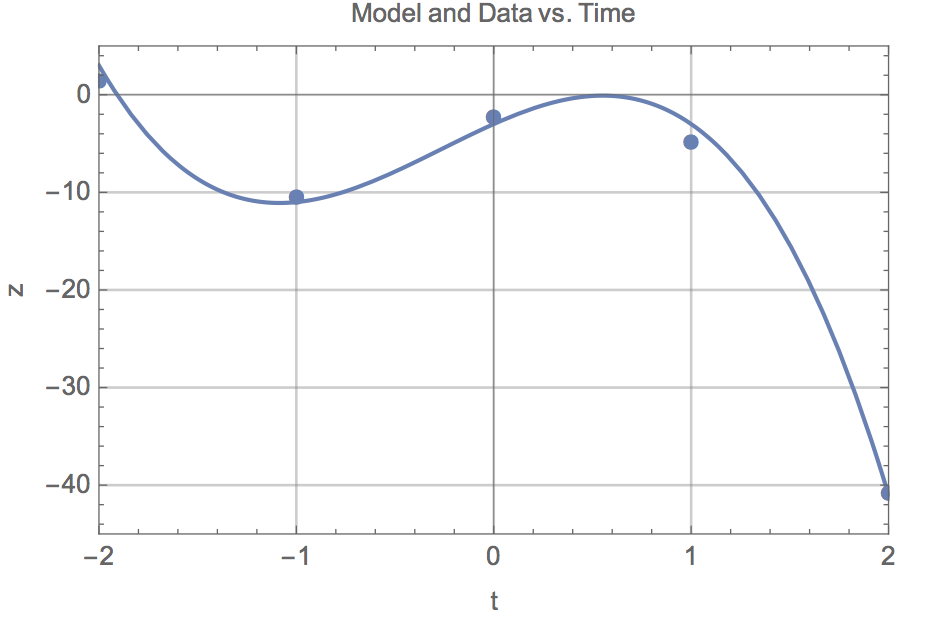
\includegraphics[width=.9\linewidth]{small_example.png}
\caption{\label{fig:orgparagraph1}
Model (solid line) and fake data (dots)}
\end{figure}

\noindent which plot as in figure \ref{fig:orgparagraph1}, where the solid line
represents the true model only the oracle knows, and the dots represent the
noisy observations the oracle gives you. Your job is to estimate the states
\(\mathbold{x}\) so that your polynomial gets as close to the oracle's as the data
allow. You must also produce the running covariance\footnote{We use the terms \emph{covariance} for matrices and \emph{variance} for scalars.} matrix
\(\mathbold{P}\) along with the states so that we have a measure of their
uncertainty.

You think for a \emph{very} long time, remembering everything you learned above, and
eventually realize that the following \texttt{cume} will do it:

\begin{verbatim}
cume[Zeta_][{x_, P_}, {A_, z_}] :=
 Module[{D, K},
  D = Zeta + A.P.Transpose[A];
  K = P.Transpose[A].Inverse[D];
  {x + K.(z - A.x), P - K.D.Transpose[K]}]
\end{verbatim}

\noindent where all quantities are matrices and the lower dot is Wolfram's matrix
multiplication.  Specifically:

\begin{itemize}
\item \(\mathbold{Z}\) is a \(1\times{1}\) matrix, the covariance of
observation noise
\item \(\mathbold{x}\) is a column \(4\)-vector, the model states
\item \(\mathbold{P}\) is a \(4\times{4}\) matrix, the theoretical
covariance of \(\mathbold{x}\)
\item \(\mathbold{A}\) is a row \(4\)-vector, the \emph{observation partials}
\item \(\mathbold{z}\) is a \({1}\times{1}\) matrix, effectively a scalar
\item \(\mathbold{D}\) is a \({1}\times{1}\) matrix, generalization of the
\emph{denominator} \(D\) we defined above in Prelude \#3
\item \(\mathbold{K}\) is a column \(4\)-vector, the \emph{Kalman gain}, generalization of the
gain \(K\) from Prelude \#3
\end{itemize}

\begin{enumerate}
\item Dimensional Arguments
\label{sec:orgheadline13}

\noindent Recall Prelude \#3, where \(D\) is \(Z+P\). We see it here as
\(\mathbold{Z}+\mathbold{A}\,\mathbold{P}\,\mathbold{A}^\intercal\). We didn't see
\(\mathbold{A}\) previously because our observations \(z\) were equal to the
states. However, here we need two factors of
\(\mathbold{A}\) to make the dimensions work out. We mean ``dimensions'' in two
senses:

\begin{enumerate}
\item dimensions of the matrices, as in numbers of rows and columns
\item physical dimensions of units of measure when \(\mathbold{z}\) and
\(\mathbold{x}\) denote physical quantities, as in most applications.
\end{enumerate}

We see another factor of
\(\mathbold{A}\) in  \(\mathbold{K}\), again required by
dimensional analysis. 

The requirement of dimensional consistency almost forces this Kalman
accumulator function. 
Here is the full dimensional breakdown. If the physical and matrix dimensions of 
\(\mathbold{x}\) 
are
\(\left[\left[\mathbold{x}\right]\right]
\stackrel{\text{\tiny def}}{=}
(\mathcal{X}, n\times{1})\)
and of 
\(\mathbold{z}\) 
are
\(\left[\left[\mathbold{z}\right]\right]
\stackrel{\text{\tiny def}}{=}
(\mathcal{Z}, b\times{1})\), then

\begin{equation*}
\label{eqn:dimensional-breakdown}
\begin{array}{lccccr}
\left[\left[\mathbold{Z}\right]\right]                                       &=& (&\mathcal{Z}^2            & b\times{b}&) \\
\left[\left[\mathbold{A}\right]\right]                                       &=& (&\mathcal{Z}/\mathcal{X}  & b\times{n}&) \\
\left[\left[\mathbold{P}\right]\right]                                       &=& (&\mathcal{X}^2            & n\times{n}&) \\
\left[\left[\mathbold{A}\,\mathbold{P}\,\mathbold{A}^\intercal\right]\right] &=& (&\mathcal{Z}^2            & b\times{b}&) \\
\left[\left[\mathbold{D}\right]\right]                                       &=& (&\mathcal{Z}^2            & b\times{b}&) \\
\left[\left[\mathbold{P}\,\mathbold{A}^\intercal\right]\right]               &=& (&\mathcal{X}\,\mathcal{Z} & n\times{b}&) \\
\left[\left[\mathbold{K}\right]\right]                                       &=& (&\mathcal{X}/\mathcal{Z}  & n\times{b}&)
\end{array}
\end{equation*}

\noindent In all examples in this paper, the observations \(\mathbold{z}\) are
\(1\times{1}\) matrices, equivalent to scalars, so \(b=1\), but the theory and code
carry over to multi-dimensional vector observations.

We can see \emph{by inspection} that the dimensions of the 
estimate\footnote{We sometimes use the center dot or the \(\times\) symbols to clarify
matrix multiplication. They have no other significance and we can always write
matrix multiplication just by juxtaposing the matrices.}
\(\mathbold{x}+\mathbold{K}\cdot(\mathbold{z}-\mathbold{A}\,\mathbold{x})\)
and the  covariance
\(\mathbold{P}-\mathbold{K}\,\mathbold{D}\,\mathbold{K}^\intercal\) are minimal
and correct.
This ``correct-by-inspection'' formulation is invaluable for checking
mathematics and code.

\item Lambda Lifting \(\mathbold{Z}\)
\label{sec:orgheadline14}

This \texttt{cume} \emph{lambda lifts}\footnote{\url{https://en.wikipedia.org/wiki/Lambda_lifting}} the observation covariance \(\mathbold{Z}\) because
it's constant for the lifetime of the filter. This means that you must
call this \texttt{cume} once with a \(\mathbold{Z}\) to get the accumulator function.
We've introduced one extra level of function-ness to avoid either
\begin{itemize}
\item coupling \texttt{cume} to an external value of \(\mathbold{Z}\) that is,
\emph{closing}\footnote{\url{https://en.wikipedia.org/wiki/Closure_(computer_programming)}} over \(\mathbold{Z}\) (we insist on pure functional coupling
only)
\item passing around a constant \(\mathbold{Z}\) in every observation packet \texttt{\{A, z\}}.
Below, where we allow \(\mathbold{Z}\) to change with each observation, we will
put it in the observation packet.
\end{itemize}

\item Folding the Accumulator Function
\label{sec:orgheadline15}

The effect of a \emph{Fold} or \emph{FoldList} with this \texttt{cume} is to incrementally
replace the prior estimate, \(\mathbold{x}\), with 
\(\mathbold{x} +
\mathbold{K}\cdot
\left(
\mathbold{z}- 
\mathbold{A}\, 
\mathbold{x} 
\right)\) 
and to replace the prior covariance, \(\mathbold{P}\), with 
\(\mathbold{P}-
\mathbold{K}\,
\mathbold{D}\,
\mathbold{K}^\intercal\). 

Here is this \texttt{cume} in action. Assume an observation-noise covariance of \(1\). Our
initial estimate for \(\mathbold{x}\) is the column vector
\(\begin{bmatrix}0& 0& 0& 0\end{bmatrix}^\intercal\),
meaning we
know nothing, and our initial state covariance is a `practical' infinity of
\(1,000\) on the diagonal, emphasizing that we know nothing. 

\begin{equation*}
\mathbold{P}_0 =
\begin{bmatrix}
 1000. & 0. & 0. & 0. \\
 0. & 1000. & 0. & 0. \\
 0. & 0. & 1000. & 0. \\
 0. & 0. & 0. & 1000. \\
\end{bmatrix}
=1000. \times \mathbold{1}_{4\times{4}}
\end{equation*}

Use \emph{Fold} rather than \emph{FoldList} because we want just the final result. \texttt{Chop}
removes quantities within a floating-point quantum of zero.

\begin{verbatim}
Fold[cume[IdentityMatrix[1]],
  {ColumnVector[{0, 0, 0, 0}], IdentityMatrix[4]*1000.0},
  {{{{1,  0., 0.,  0.}}, { -2.28442}}, 
   {{{1,  1., 1.,  1.}}, { -4.83168}}, 
   {{{1, -1., 1., -1.}}, {-10.46010}}, 
   {{{1, -2., 4., -8.}}, {  1.40488}}, 
   {{{1,  2., 4.,  8.}}, {-40.8079}}}
  ] // Chop
~~>
\end{verbatim}

\begin{align}
\label{eqn:kalman-filter-results}
\mathbold{x} &=
\begin{bmatrix}
 -2.97423 \\
  7.2624  \\
 -4.21051 \\
 -4.45378 \\
\end{bmatrix}
\\
\notag
\mathbold{P} &=
\begin{bmatrix}
 0.485458 & 0 & -0.142778 & 0 \\
 0 & 0.901908 & 0 & -0.235882 \\
 -0.142778 & 0 & 0.0714031 & 0 \\
 0 & -0.235882 & 0 & 0.0693839 \\
\end{bmatrix}
\end{align}

\begin{figure}[htb]
\centering
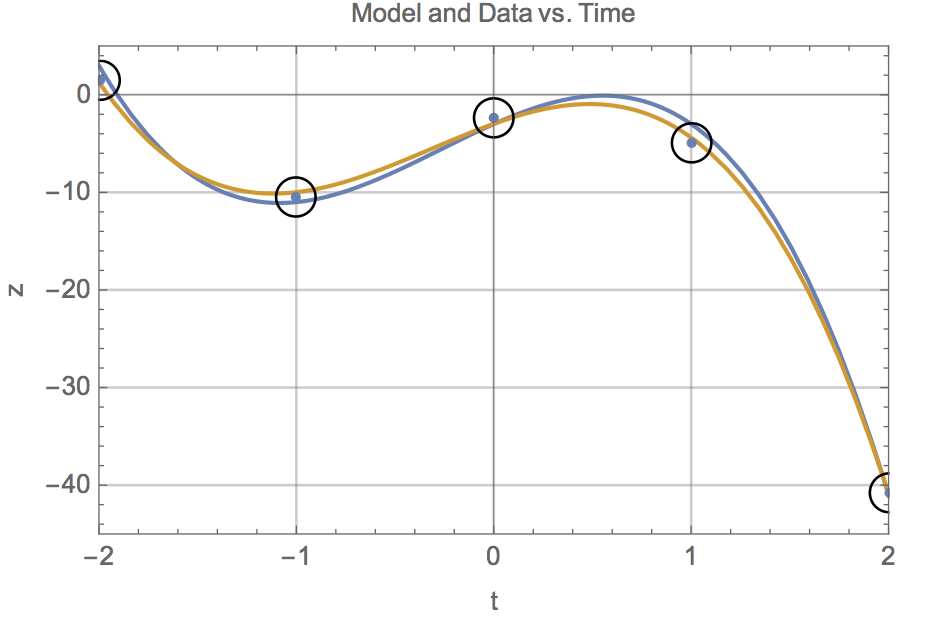
\includegraphics[width=.9\linewidth]{small_solution.png}
\caption{\label{fig:orgparagraph2}
Model (dark line), fake data (dots), and estimated model (light line)}
\end{figure}

Results are not bad: our oracle reveals that ground-truth is
\(\begin{bmatrix}-3& 9& -4& -5\end{bmatrix}^\intercal\); compare
this to equation \ref{eqn:kalman-filter-results}.
Figure \ref{fig:orgparagraph2} plots the solution.

To find out quantitatively how bad or how good,  inspect
\(\mathbold{P}\). Its diagonal elements are the squares of the
standard deviations of the estimated states. Those standard deviations are:

\begin{equation*}
\begin{bmatrix}
0.6967 & 0.9497 & 0.2672 & 0.2634
\end{bmatrix}
^\intercal
\end{equation*}

All our estimates are within two standard deviations of
ground truth, so we would expect worse performance in only \(5\) percent of
cases.
\end{enumerate}

\subsection{Kalman is a Swiss-Army Knife}
\label{sec:orgheadline18}

This is remarkable. An accumulator function, small enough to fit on a business
card, suffices to estimate states of \emph{any} linear model in constant memory. It
does not need data to get started, just \emph{a-priori} guesses, even vacuous ones.
Its code fits on tiny embedded systems. It empowers radar, navigation,
tracking, the entire space age, industrial robotics, battery-charge estimation,
radio interferometry, econometrics. It can be extended to non-static and
nonlinear models, to non-scalar observations, and to non-Gaussian noise sources.
It's the sweet spot in a spectrum of statistical estimators that progress from
counting to Markov-chain Monte Carlo (MCMC) filters.\footnote{\url{https://en.wikipedia.org/wiki/Particle_filter}}

\subsection{More Intuition}
\label{sec:orgheadline19}

In \emph{ex-post-facto} justification for choosing the Wolfram language,
it allows the code above to look very similar to the
mathematical specification:

\begin{equation}
\label{eqn:kalman-cume-definition}
\text{cume}
\left(
\mathbold{Z}
\right)
\left(
\left\{
\mathbold{x},
\mathbold{P}
\right\},
\left\{
\mathbold{A},
\mathbold{z}
\right\}
\right) =
\left\{
\mathbold{x}+
\mathbold{K}\,
\left(
\mathbold{z}-
\mathbold{A}\,
\mathbold{x}
\right),
\mathbold{P}-
\mathbold{K}\,
\mathbold{D}\,
\mathbold{K}^\intercal
\right\}
\end{equation}

\noindent where

\begin{align}
\label{eqn:kalman-gain-definition}
\mathbold{K}
&=
\mathbold{P}\,
\mathbold{A}^\intercal\,
\mathbold{D}^{-1} \\
\label{eqn:kalman-denominator-definition}
\mathbold{D}
&= \mathbold{Z} +
\mathbold{A}\,
\mathbold{P}\,
\mathbold{A}^\intercal
\end{align}

A good way to intuit this solution is to think of \(\mathbold{K}\) as the derivative
\(\text{d}\mathbold{x}/\text{d}\mathbold{z}\). We've already seen that the
physical dimensions of \(\mathbold{K}\) are the required
\(\mathcal{X}/\mathcal{Z}\). Then, the update resembles

\begin{equation*}
\mathbold{x}
\leftarrow
\mathbold{x} +
\diff{\mathbold{x}}{\mathbold{z}}
\left(
\mathbold{z}-
\mathbold{A}\,
\mathbold{x}
\right)
\end{equation*}

\noindent which looks like a differential update to the estimate
\(\mathbold{x}\), where the differential of \(\mathbold{z}\) is the residual
difference between an actual observation \(\mathbold{z}\) and a prediction of
\(\mathbold{z}\) from the current model partials matrix \(\mathbold{A}\) times the
prior estimate \(\mathbold{x}\).

The gain \(\text{d}\mathbold{x}/\text{d}\mathbold{z}\) has the form, in a slight
abuse of notation:

\begin{equation*}
\mathbold{K}=
\frac{
\mathbold{P}\,
\mathbold{A}^\intercal
}{
\mathbold{Z}+
\mathbold{A}\,
\mathbold{P}\,
\mathbold{A}^\intercal
}
\end{equation*}

An elegant but non-trivial derivation of this appears in a separate paper in this 
series.\footnote{Beckman, \emph{Kalman Folding 3: Derivations}, to appear.} 
Just remember that the \emph{denominator matrix},
\(\mathbold{D}\), is \(\mathbold{Z}\) \emph{plus} a correction. Likewise, I do not know
an easy demonstration that the new \(\mathbold{P}\) is the old \(\mathbold{P}\)
minus \(\mathbold{K}\,\mathbold{D}\,\mathbold{K}^\intercal\). In this case, just
remember the \emph{minus} sign. Intuitively, it's plausible that the new
\(\mathbold{P}\) should be `less than' the old \(\mathbold{P}\) because the new
observations add information and decrease uncertainty. That plausibility
motivates the minus sign in the formula.

\section{Functional Form Encapsulates Code}
\label{sec:orgheadline21}

We stated above that we can run \emph{exactly} the same Kalman code over lazy streams
and over asynchronous observables. This is possible because the only coupling
between the environment and the Kalman code is function invocation.

Why is this important? Because developers can test in friendly environments ---
where observations are deterministic, pseudo-random, static, present in memory
all at once, and where code can be stopped in a debugger. Once the code is
hardened, developers can then deploy it with confidence in unfriendly,
real-world environments --- where data are unpredictable, asynchronous,
real-time, infinite in length, and logging is the only forensic tool.

This advantage can be critically important when detecting, diagnosing, and
correcting numerical issues like catastrophic cancellation, as we see in the
calibration example below. Numerical issues can substantially complicate code,
and being able to move exactly the same code, without even recompiling, between
testing and deployment can make the difference to a successful application. We
have seen many cases where differences in compiler flags, let alone differences
in architectures, even between different versions of the same CPU family,
introduce enough differences in the generated code to cause qualitative
differences in the output. A filter that behaved well in the lab can fail in practice. In
embedded applications like tracking and navigation, filter failure can cause
vehicles to crash. It \emph{must} be caught in testing and it must \emph{not} be allowed
to happen in deployment.

\section{An Instrument-Calibration Example}
\label{sec:orgheadline26}

Imagine an accelerometer that comes from the factory with unknown bias, scale,
and drift errors. The user's manual instructs us to calibrate the instrument
before fielding. That means estimating these errors so that we can subtract
their effects in post-processing. 

In this example, we allow the observation covariance \(\mathbold{Z}\) to vary with
independent variable, so we don't lambda-lift \(\mathbold{Z}\), but pass it into
the filter each step along with \(\mathbold{A}\) and \(\mathbold{z}\).

\subsection{Functional Form, Again}
\label{sec:orgheadline22}

Because the values of these errors are small, their variances, by squaring, are
even smaller, and we invite catastrophic cancellation into the filter, on
purpose. We verified numerically that in all examples above, three,
mathematically equivalent expressions for the covariance, namely

\begin{align*}
\mathbold{P} &\leftarrow
\mathbold{L}\,
\mathbold{P} 
\\
\mathbold{P} &\leftarrow
\mathbold{L}\,
\mathbold{P}\,
\mathbold{L}^\intercal +
\mathbold{K}\,
\mathbold{Z}\,
\mathbold{K}^\intercal
\\
\mathbold{P} &\leftarrow
\mathbold{P} -
\mathbold{K}\,
\mathbold{D}\,
\mathbold{K}^\intercal
\end{align*}

\noindent produce results identical to six significant 
figures.\footnote{Derivations of these forms appear in part 3 of this series.} 
This means high
confidence that numerical issues are not important in these examples.

However, in the present example, all three expressions produce different
results: two converge with different numerical details, and one fails. The first
two occasionally produce negative covariances, and the third produces mostly
negative covariances, exhibiting catastrophic cancellation.

Once a covariance produces bad values, the estimates soon follow because the
covariance feeds back through
\(\mathbold{D}=\mathbold{Z}+\mathbold{A}\,\mathbold{P}\,\mathbold{A}^\intercal\)
and then into \(\mathbold{K}=\mathbold{P}\,\mathbold{A}^\intercal/\mathbold{D}\).
Once \(\mathbold{K}\) destabilizes, the estimates
\(\mathbold{x}\leftarrow\mathbold{x}+\mathbold{K}(\mathbold{z}-\mathbold{A}\,\mathbold{x})\)
quickly become nonsense.

This example was adapted from Zarchan and Musoff.\footnote{Zarchan and Musoff, \emph{Fundamentals of Kalman Filtering, A Practical
Approach, Fourth Edition}, Ch. 4} We verified
numerically that one of our examples matches their results, including negative
variances, to six significant figures. Presumably because their code eventually
converged, they didn't discuss catastrophic cancellation, but we focus on it
here.

\subsection{Details of the Example}
\label{sec:orgheadline23}

The documented calibration procedure is to hold the accelerometer vertically at
a sequence of angles from \(0\) degrees to \(180\) degrees in \(2\)-degree
increments, allowing Earth's gravitation to provide a fiducial acceleration.
Measure the output of the accelerometer and compare it to a theoretical model
that depends on the bias, scale, and drift errors. The model is linear, so the
procedure is a perfect prescription for a Kalman filter.

Let the angle of the accelerometer with respect to the vertical be \(\theta\). The
accelerometer documentation dictates that the output should read

\begin{align}
a &= g \,\cos(\theta) + z \\
\label{eqn:accelerometer-observations}
z &= b + s\, g\, \cos(\theta) + d\, g^2 \,\cos^2(\theta)
\end{align}

\noindent where we observe \(z\) and

\begin{center}
\begin{tabular}{lll}
\(g=\) & acceleration of Earth's gravitation & \(\sim 32.2 \,\textrm{foot}/\textrm{sec}^2\)\\
\(b=\) & bias & \(\textrm{foot} / \textrm{sec}^2\)\\
\(s=\) & scale & dimensionless\\
\(d=\) & drift & \(\textrm{sec}^2 / \textrm{foot}\)\\
\end{tabular}
\end{center}

Our vector of states is
\(\mathbold{x}=\begin{bmatrix}b&s&d\end{bmatrix}^\intercal\) and our partials are
\(\mathbold{A}(\theta)=\begin{bmatrix}1&gc_\theta&g^2c^2_\theta\end{bmatrix}\)

\noindent where \(c_\theta=\cos(\theta)\). 

Our measurement rig delivers noisy angles, not noisy values of \(\cos(\theta)\),
so we must translate angle noise \(\zeta_\theta\), of constant variance
\(\sigma_\theta^2\), into \(c_\theta\) noise \(\zeta_{c_\theta}\) with a variable
variance \(\sigma_{c_\theta}\), and then into observation noise \(\zeta_z\) with
variance \(\mathbold{Z}(\theta)\). We find

\begin{equation}
\mathbold{Z}(\theta) = \left(\sigma_\theta\,g\,\sin(\theta)\right)^2 
\end{equation}

Posit a ground truth for \(\mathbold{x}\) of 

\begin{equation}
\mathbold{\aleph} =
\begin{bmatrix}
10\times{10^{-6}}\,g \\
5\times{10^{-6}}\\
1\times{10^{-6}}/g
\end{bmatrix}
\end{equation}

\noindent and generate deterministic pseudo-randomly noisy observations as
follows:

\begin{equation}
\mathbold{A}(\theta)\cdot\aleph + g\,(\cos(\theta + \zeta_\theta) -\cos(\theta))
\end{equation}

\subsection{Results}
\label{sec:orgheadline24}

\begin{figure}[htb]
\centering
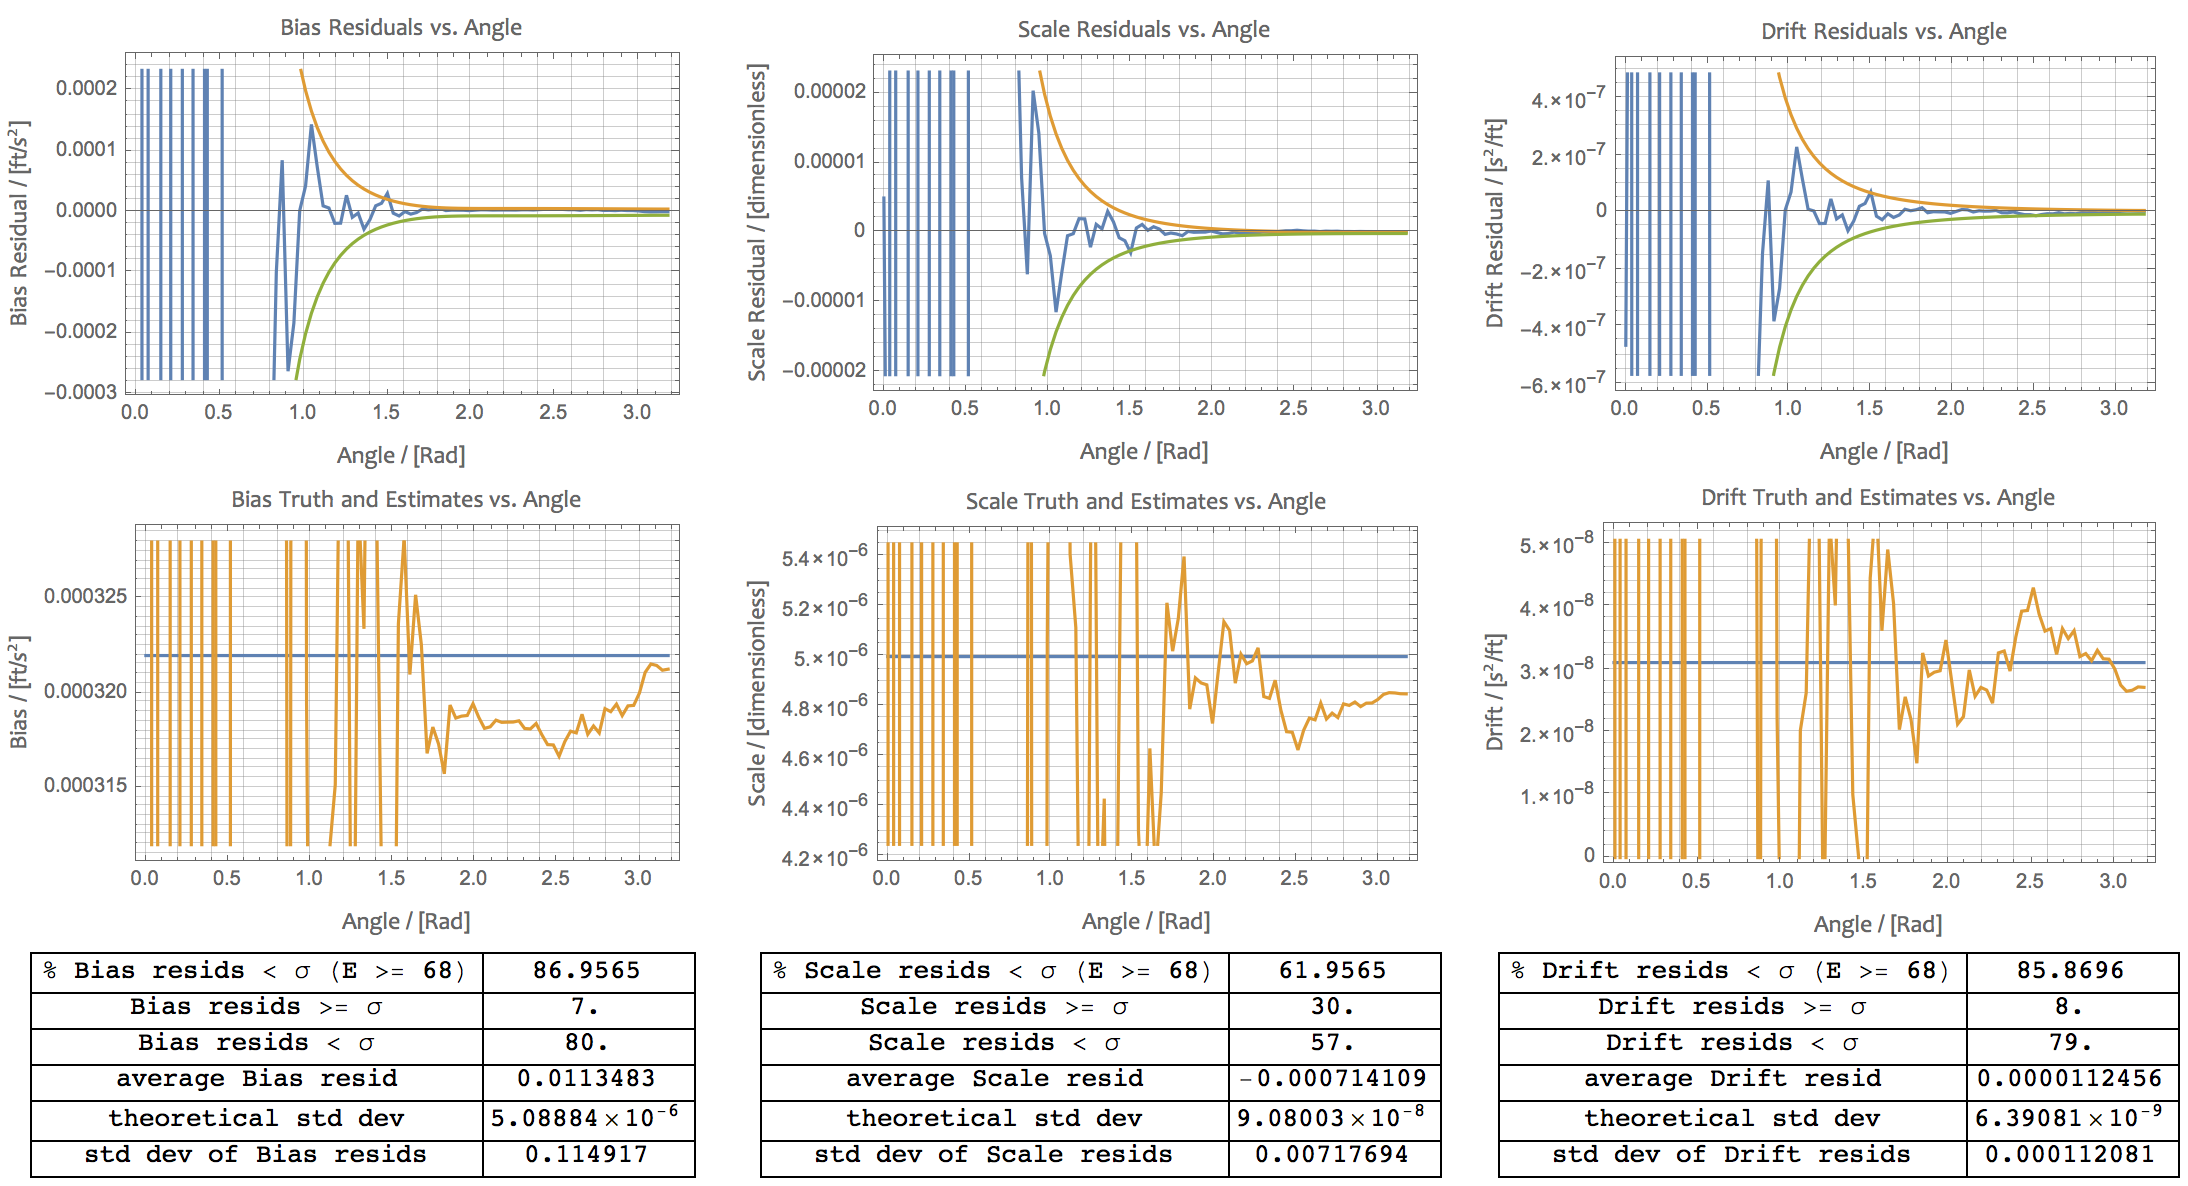
\includegraphics[width=.9\linewidth]{zarchan_musoff_1.png}
\caption{\label{fig:orgparagraph3}
Accelerometer calibration results, \(\mathbold{P}\leftarrow\mathbold{L}\,\mathbold{P}\)}
\end{figure}

We test three mathematically identical Kalman accumulator functions, 
differing only in their formula for \(\mathbold{P}\). The first, illustrated in
figure \ref{fig:orgparagraph3}, reproduces Zarchan and Musoff to six significant
figures, including occasional negative variances. This produces acceptable
results, near ground truth. Zarchan and Musoff's code for the filter is
fully enmeshed with their code for constructing and delivering 
observations, so there is no hope of extracting it without change into a
deployment environment. Not so our code, which we can harden and move verbatim,
according to the main message of this paper.

\begin{verbatim}
kalman[{x_, P_}, {Zeta_, A_, z_}] :=
  Module[{D, K, L},
   D = Zeta + A.P.Transpose[A];
   K = P.Transpose[A].inv[D];
   L = (id[len[P]] - K.A);
   {x + K.(z - A.x), L.P}]; 
                     (* also L.P.Transpose[L] + K.Zeta.Transpoe[K] *)
                     (* or   P - K.D.Transpose[K] *)
\end{verbatim}

\begin{figure}[htb]
\centering
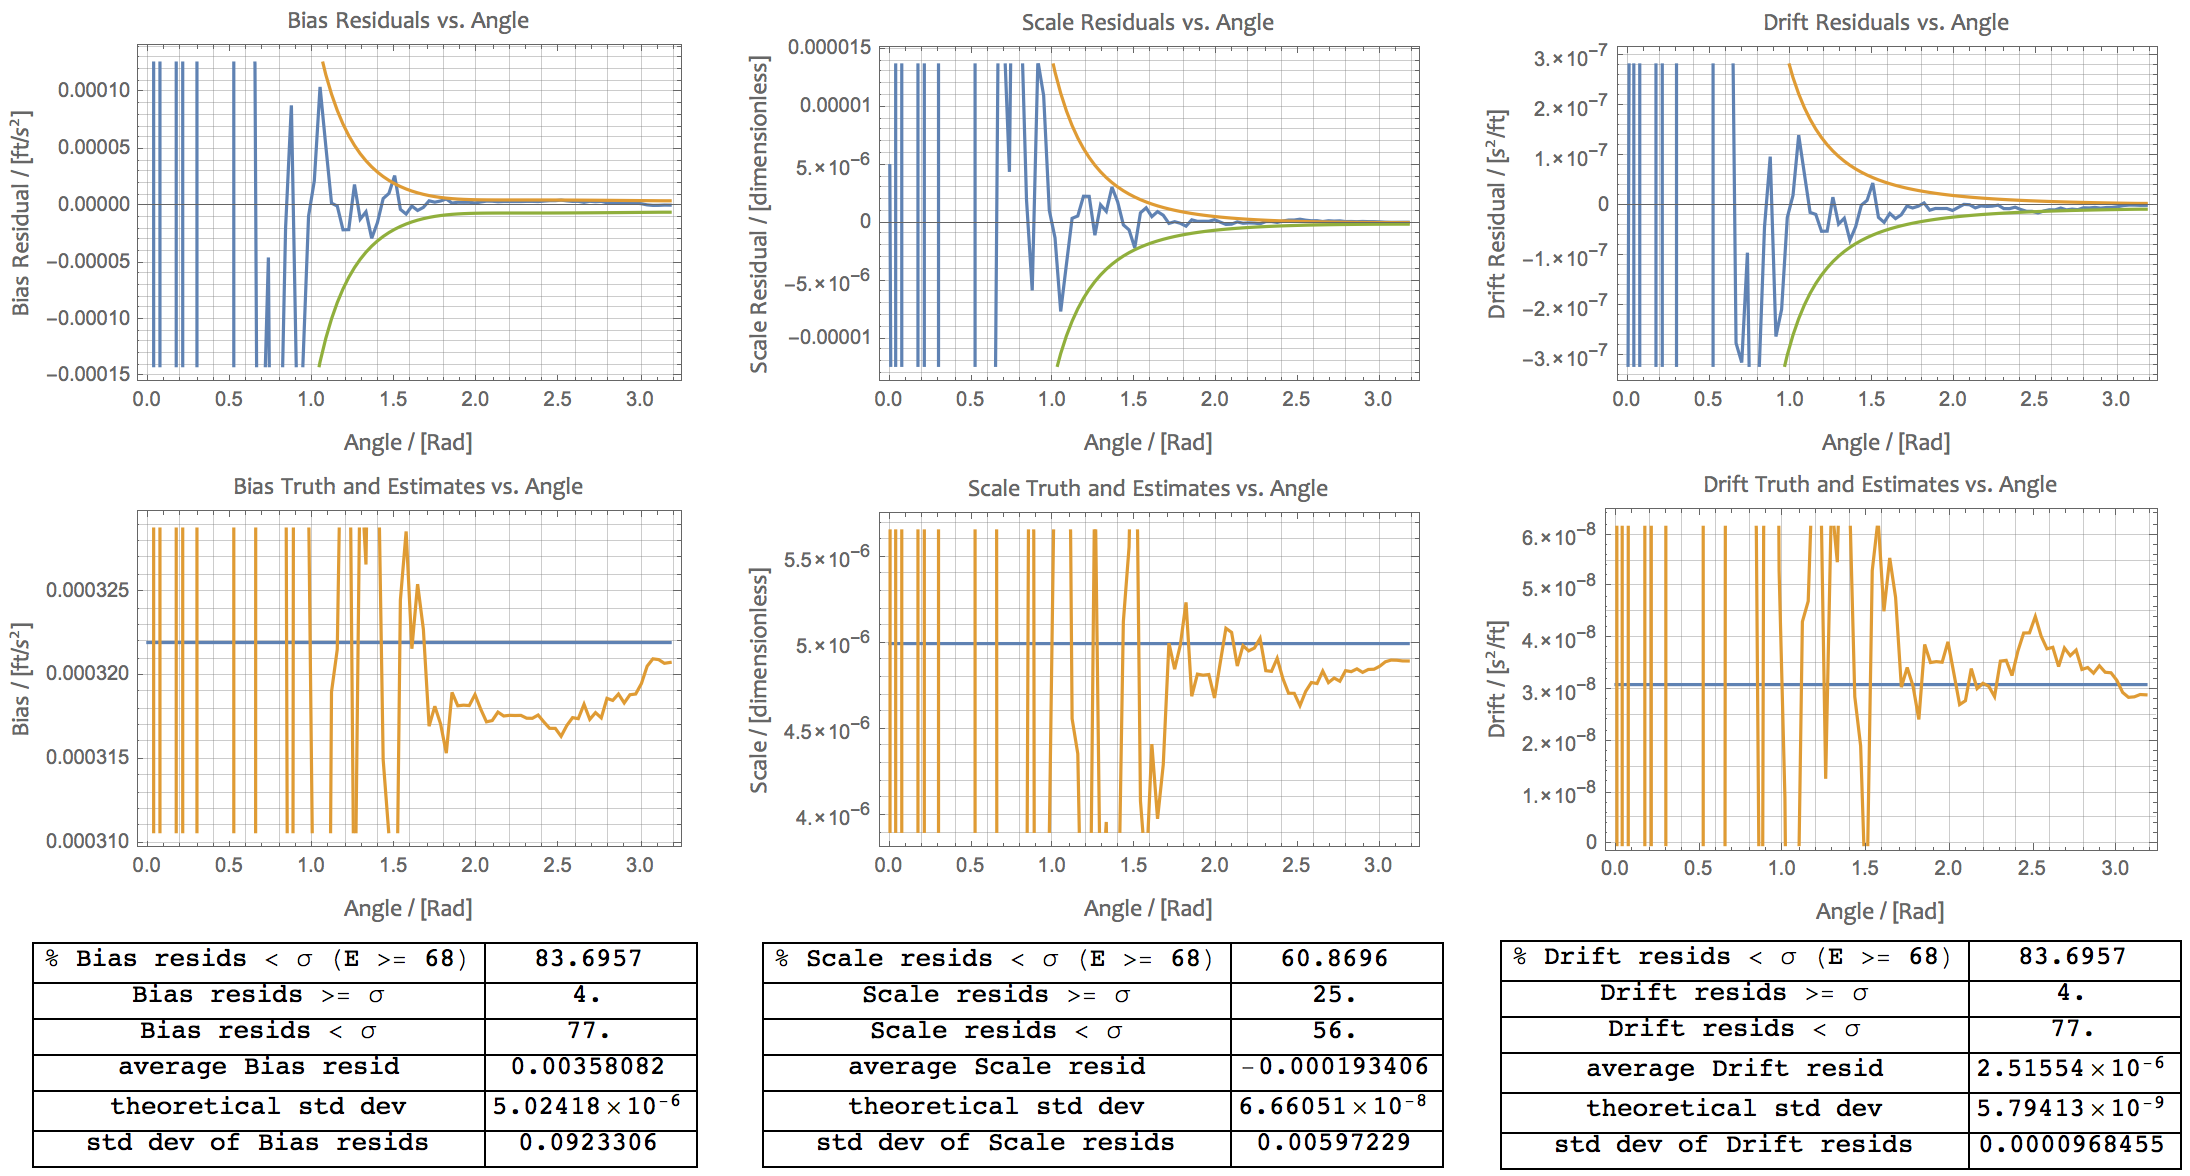
\includegraphics[width=.9\linewidth]{zarchan_musoff_2.png}
\caption{\label{fig:orgparagraph4}
Accelerometer calibration results, \(\mathbold{P} \leftarrow\mathbold{L}\,\mathbold{P}\,\mathbold{L}^\intercal +\mathbold{K}\,\mathbold{Z}\,\mathbold{K}^\intercal\)}
\end{figure}

The second filter produces similar and acceptable results but with totally
different numerical values even with exactly the same pseudo-random fakes. This
is illustrated in figure \ref{fig:orgparagraph4}. Tracking down the sources of
these numerical differences would require a deep numerical study, but might
be necessary in a safety-critical or mission-critical application.

\begin{figure}[htb]
\centering
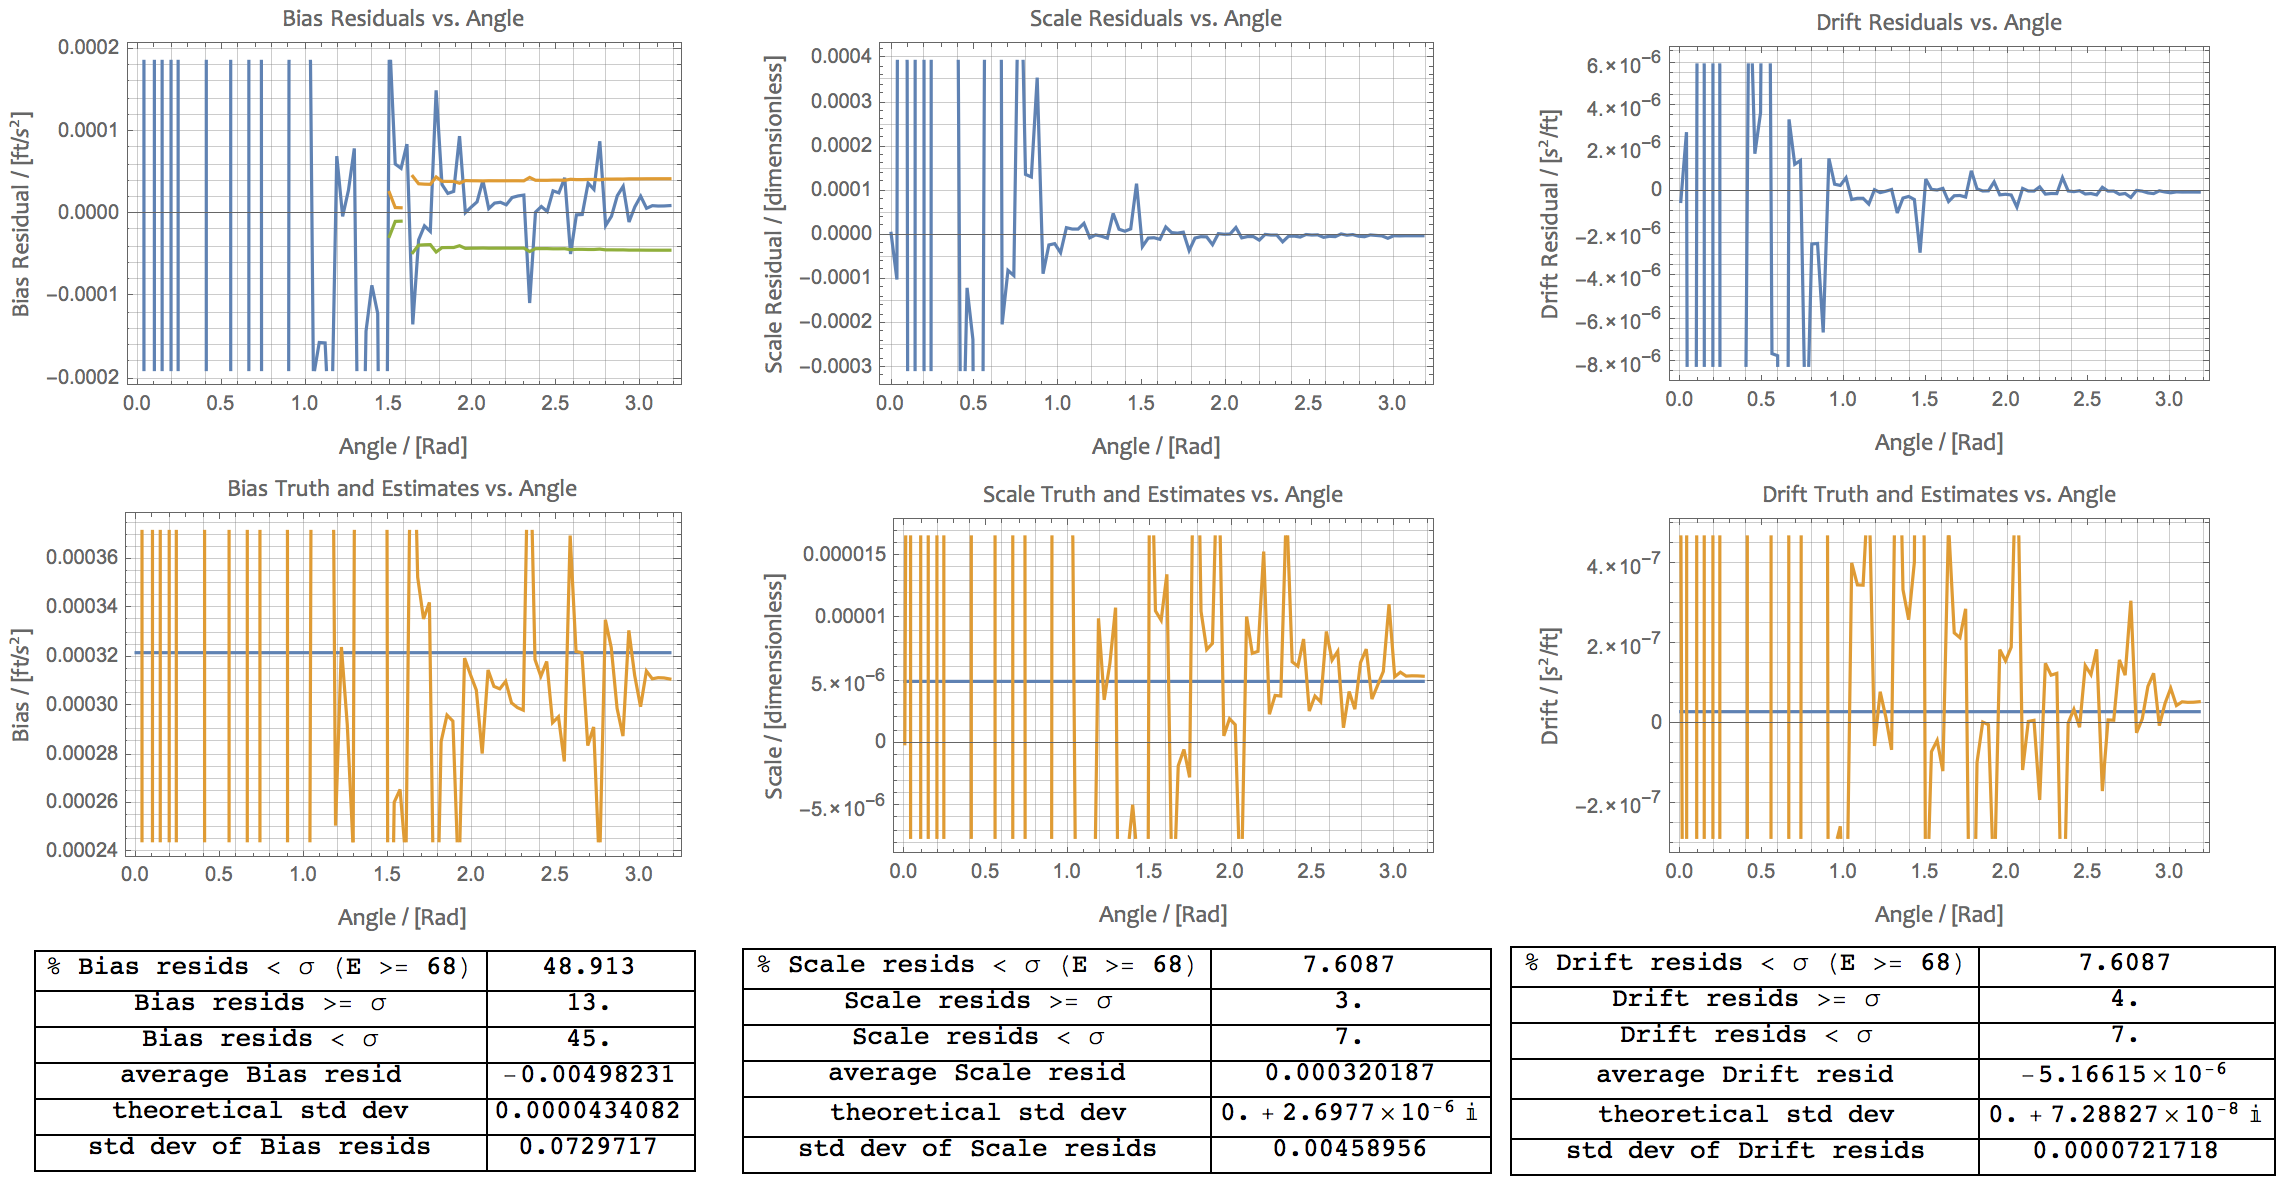
\includegraphics[width=.9\linewidth]{zarchan_musoff_3.png}
\caption{\label{fig:orgparagraph5}
Accelerometer calibration failure, \(\mathbold{P}\leftarrow\mathbold{P} -\mathbold{K}\,\mathbold{D}\,\mathbold{K}^\intercal\)}
\end{figure}

We would be advised to move to the SRIF family of filters after seeing this much
variability, but even more so after the third filter, our original Kalman fold,
fails, as illustrated in figure \ref{fig:orgparagraph5}. Remarkably, despite
meaningless covariances, the estimates are still reasonable compared to ground
truth, but they certainly cannot be trusted.

\subsection{Robustness}
\label{sec:orgheadline25}

It is a general feature of Kalman filters that they are difficult to break in
practice. We can bend the rules, feeding them non-Gaussian noise with very large
variances, and they will often converge despite the abuse. In fact, routine
practice is to patch diverging filters with artificial process noise.
However, this example illustrates that hazards exist and should be carefully
analyzed. This is all the more reason to favor a functional form that enables
easy movement between testing and deployment.

\section{Concluding Remarks}
\label{sec:orgheadline27}

The basic Kalman filter statistically inverts the basic model

\begin{equation*}
\mathbold{z} = \mathbold{A}\,\mathbold{x}
\end{equation*}

\noindent yielding a sequence of estimates of \(\mathbold{x}\), which may
additionally evolve over time according to a linear state-transition model.

The flashes of insight required to invent the Kalman filter were really flashes
of genius. There was a lot of prior work, mostly coming from radar and the
tracking community, on incremental optimal estimation. But Kalman saw what
others did not see: that new observations could be simply scaled by covariances
and added to old. These insights enabled whole disciplines of guidance and
control that propelled the space age and all the rest of aerospace since Kalman
had them in 1960 because
\emph{we can perform state estimation fast, incrementally and in constant memory just as with other, lesser statistics like count, mean, and standard deviation.}

Writing the code for a Kalman filter as a foldable accumulator function gives us
\begin{itemize}
\item economy of expression, reducing otherwise complex and tricky code
to a few, modularized and decoupled lines
\item flexibility of testing and deployment, allowing exactly the same
code, even and especially binary, to run over arrays in
memory, lazy streams, asynchronous observables, any data source
that can support a \emph{fold} operator
\item flexibility of application, reducing the inputs to a handful
of  matrices
\end{itemize}

We hope that by illuminating this flexibility we can expand the use of the
Kalman filter into other application areas. We also hope to inspire the study
and application of more advanced filters like the Extended and Unscented Kalman
filters, Information filters and Square-Root Information filters, Sigma-Point
filters, and Particle filters.
% Emacs 24.5.1 (Org mode 8.3.4)
\end{document}